\documentclass[12pt,openany]{book}

%PACKAGES%
\usepackage[inner=25.86mm, outer=18.24mm, top=25.86mm, bottom=33.48mm, papersize={154mm, 216mm}]{geometry}
\usepackage[german]{babel}
\usepackage{graphicx}
\usepackage{fontspec}
\usepackage{enumitem}
\usepackage{sectsty}
\usepackage[]{titlesec}
\usepackage{verse}
\usepackage{fix-cm}%font size
\usepackage{multirow}%tables
\usepackage{array}%tables
\usepackage[hyphens]{url}
\usepackage[toctextentriesindented]{tocstyle}
\usepackage{tocloft}
\usepackage{soulutf8}
\usepackage{marginnote}
\renewcommand*{\marginfont}{\SkolarLight}

%this snippet of code is a bit of a hack to allow line break after em-dash (http://tex.stackexchange.com/questions/62800/lualatex-and-line-breaks-after-em-dashes)
\catcode`\—=13
\protected\def—{\unskip\textemdash\allowbreak}

%\usepackage{pagegrid}
%PACKAGES%
%\pagegridsetup{top-left, step=3.435in}

%TABLE OF CONTENTS%
\settocstylefeature[]{leaders}{\hfill}%ELIMINATES DOTS%
\settocstylefeature[0]{entryvskip}{0.5em}%VERTICAL SPA\caps{ce} BEFORE CHAPTER ENTRIES%
\renewcommand*{\cfttoctitlefont}{\Secfont\Large}%use tocloft
%TABLE OF CONTENTS%

%LINESPACE% SETS LINESPA\caps{ce}
\usepackage{setspace}
\setstretch{1.15}
%LINESPACE%

%FONTS% These are the normal SC fonts. We have a ``light'' skolar, too. 
\setmainfont[Numbers=OldStyle]{Alegreya ht Pro}
\setsansfont[Scale = MatchLowercase]{Source Sans Pro}
\setmonofont{Source Code Pro}


\newfontfamily\Chapfont[ItalicFont=Alegreya Sans Italic]{Alegreya Sans}
\chapterfont{\Chapfont\LARGE\centering\mdseries\setstretch{1}}
\newfontfamily\Secfont[Numbers=OldStyle]{Alegreya Sans Medium}
\sectionfont{\Secfont\mdseries\large\setstretch{1}}


%HEADINGS%

%HEADER% 
\usepackage{fancyhdr, textcase}
\setlength{\headheight}{15pt}
\pagestyle{fancy}
\renewcommand{\chaptermark}[1]{\markboth{\thechapter.\ #1}{}}
\renewcommand{\sectionmark}[1]{\markright{\thesection\ #1}}

\fancyhf{}
\fancyhead[LE,RO]{\thepage}
\fancyhead[CO]{\headcaps{\MakeUppercase{Ajahn Brahmali}}}
\renewcommand{\headrulewidth}{0pt}
\fancypagestyle{plain}{ %
\fancyhf{} % remove everything
\renewcommand{\headrulewidth}{0pt}
\renewcommand{\footrulewidth}{0pt}}
\newfontfamily\headcapsfont[RawFeature=+c2sc]{Alegreya ht Pro}
\newcommand\headcaps[1]{{\headcapsfont #1}}
\fancyhead[CE]{\headcaps{\MakeUppercase{Samatha \& Vipassanā}}}
%HEADER%

%HANGING LEFT%
\newcommand*{\vleftofline}[1]{\leavevmode\llap{#1}}
%HANGINGLEFT%

%WIDOWS & ORPHANS% 
\widowpenalty=10000
\clubpenalty=10000
%WIDOWS & ORPHANS%

%Applies various subtle improvements in typography. Use default.
\usepackage{microtype}
\frenchspacing

\usepackage[unicode, hidelinks, pdfauthor={Brahmali}, pdftitle={Warum Samatha und Vipassanā unzertrennlich sind}, pdfsubject={Buddhism}, pdfkeywords={Buddhismus, Bhikkhu, Mönche, Sutta, Tipitaka, Tripitaka, Sutra, Samatha, Vipassana, Ruhe, Einsicht}, pdfproducer={LuaTeX  beta-0.70.1}, pdfcreator={LaTeX2e}]{hyperref}

%DOCUMENT INFO. NOT USED IN TEXT.%
\title{Warum Samatha und Vipassanā \protect\\ unzertrennlich sind}
\author{Ajahn Brahmali}
\date{}
\begin{document}
\frontmatter
\pagestyle{empty}
\newgeometry{margin=0px}

\hspace*{-156mm}
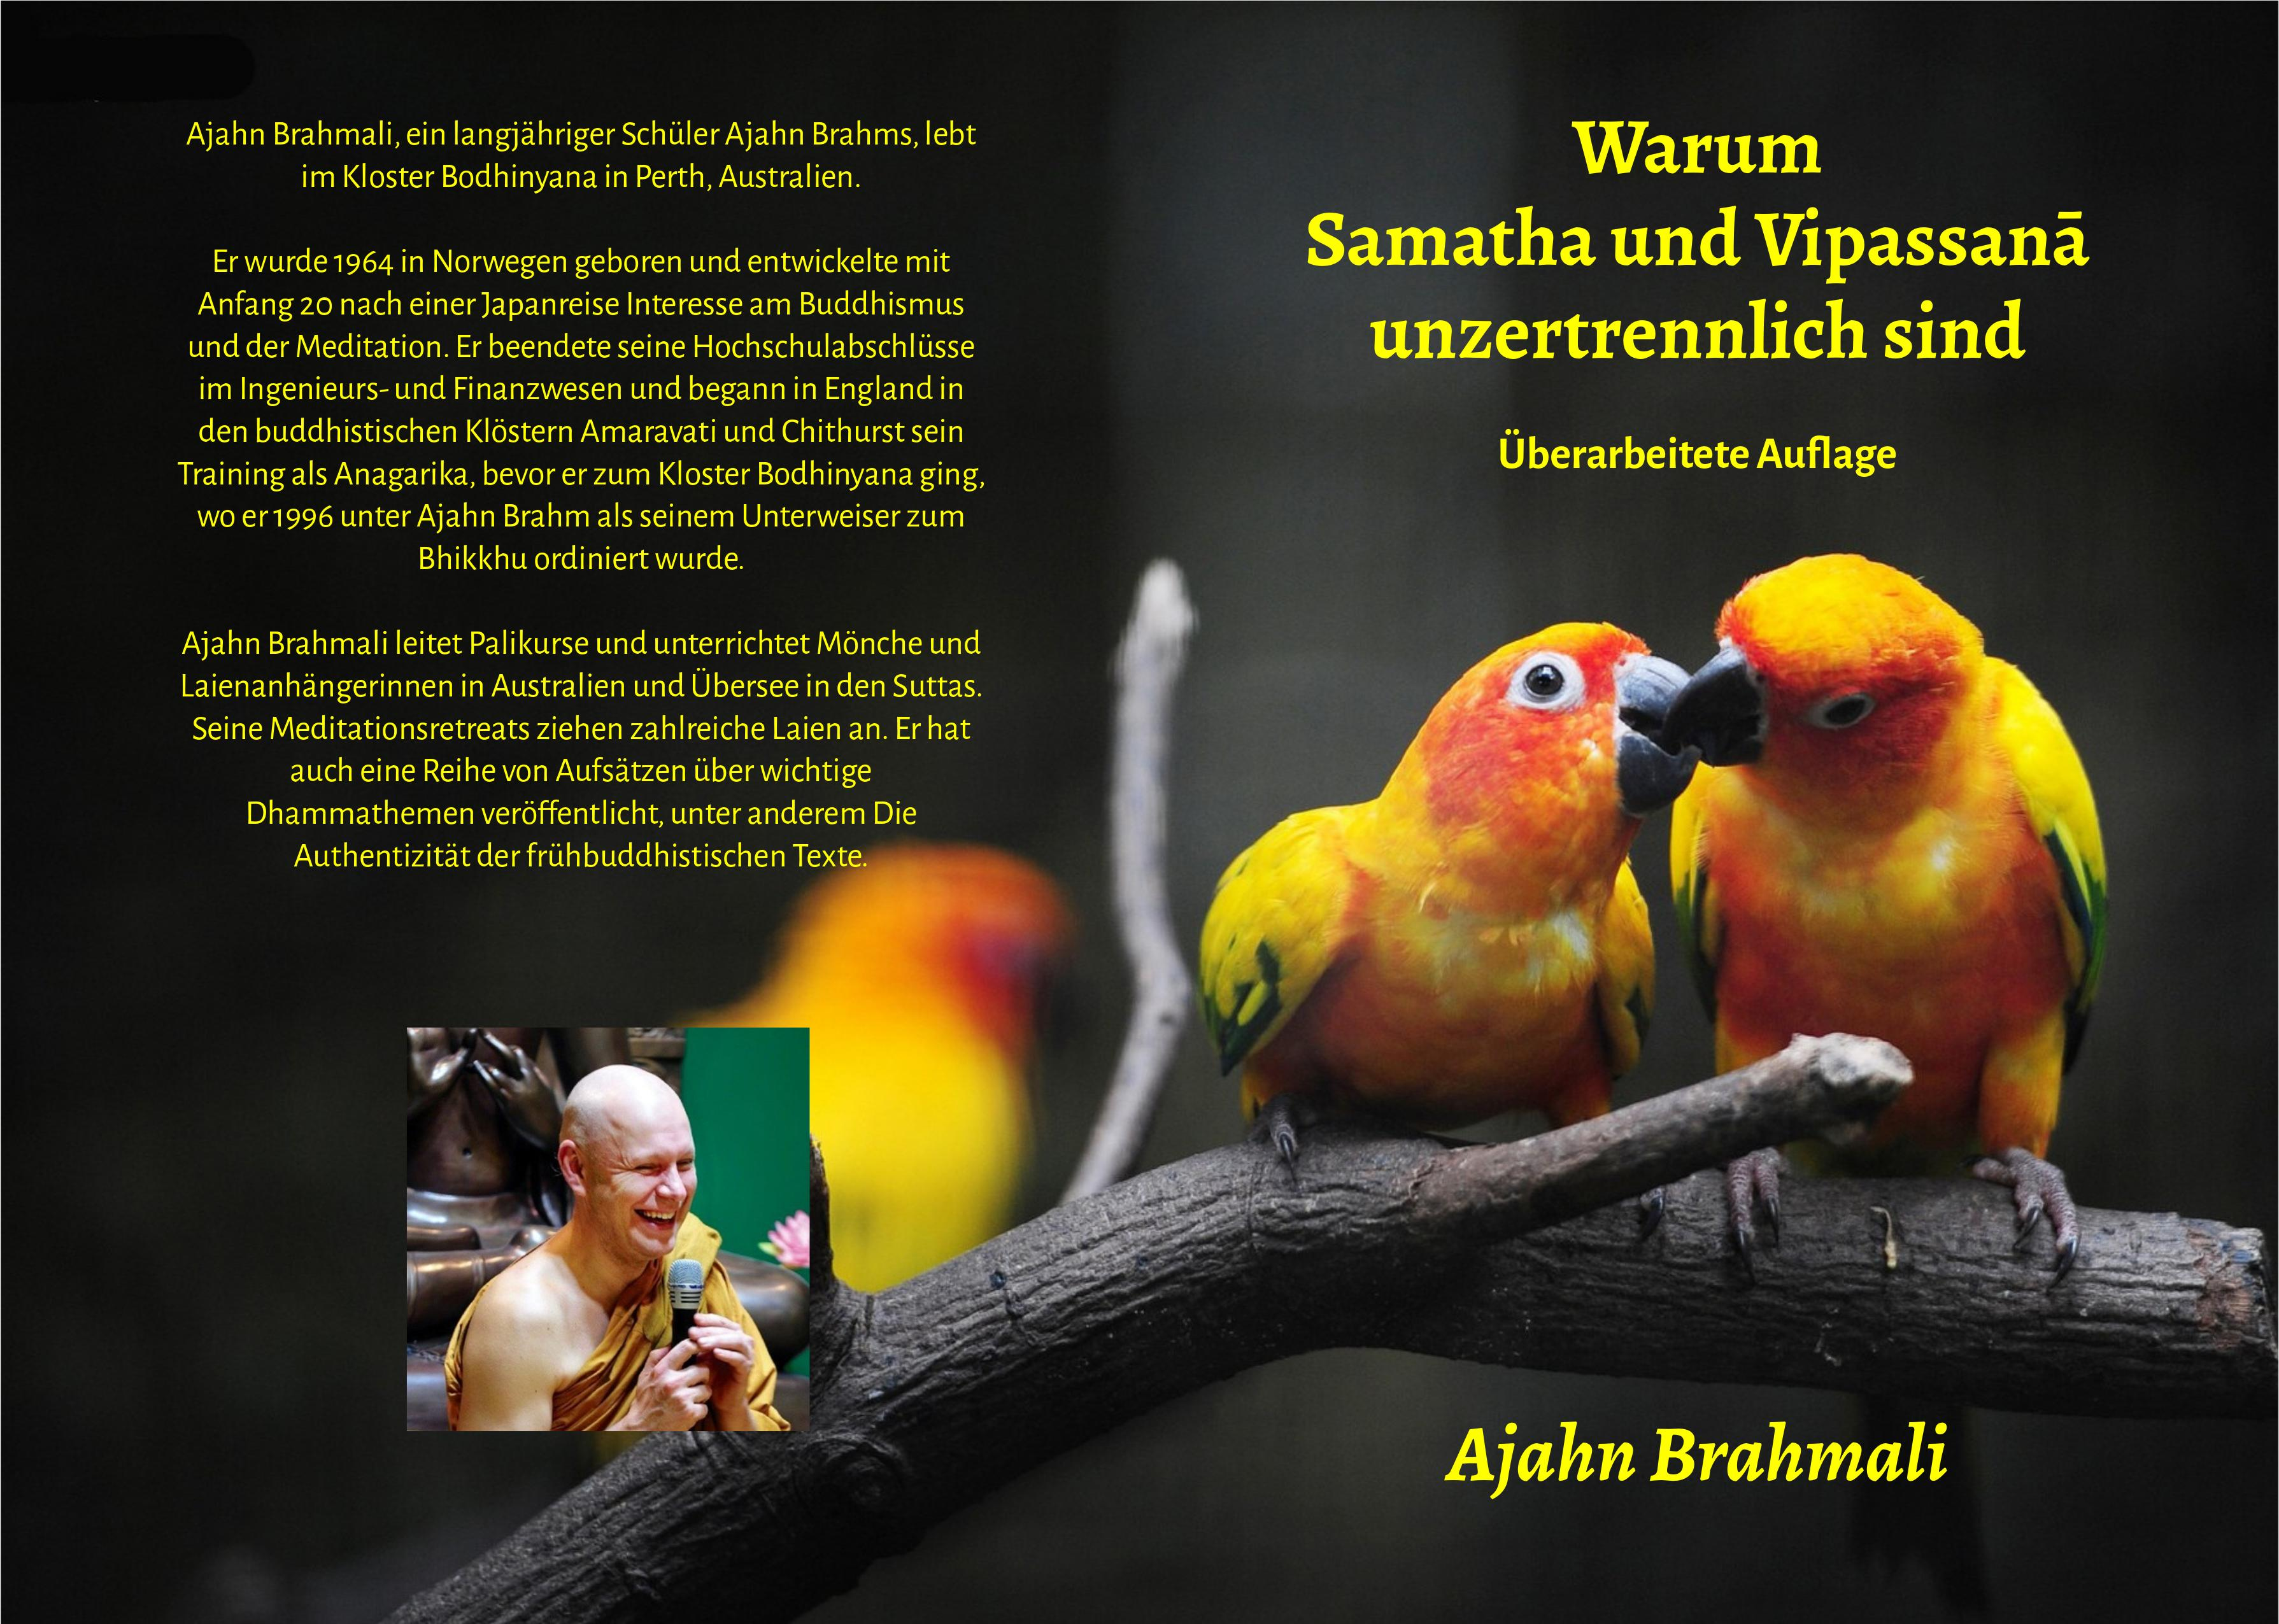
\includegraphics{sv-2_a5_cover_de-new}

\begin{center}\end{center}
\begin{center}

\vfill

\maketitle

\vfill
\end{center}

\newpage
\restoregeometry

\begin{center}\end{center}

\vspace{4em}
{\small
\noindent Auf der Grundlage eines Vortrags vom Freitag, den 8. Mai 2015 \\im buddhistischen Zentrum Dhammaloka, Perth, Australien.

\medskip

\noindent Überarbeitete Auflage

\medskip

\noindent Deutsch von Anagarika Sabbamitta

\noindent Lektorat: Bhikkhu Bodhidhaja

\medskip

\noindent \emph{Originaltitel:}

\noindent Why Samatha and Vipassanā are Inseparable
\medskip

\noindent Copyright Ajahn Brahmali
\medskip

\noindent \emph{Herausgegeben von:}

\noindent Buddhist Society of Western Australia

\noindent 18 Nanson Way, Nollamara, WA 6061, Australia

\noindent admin@bswa.org



}

\vfill

\begin{center}
\textit{Mögen alle Wesen gesund und glücklich sein!}

\end{center}
\vfill

 \newpage

\begin{center}\end{center}
\begin{center}

\vfill

{\huge \textit{Warum} 

\medskip

\textbf{Samatha} \textit{und} \textbf{Vipassanā} 

\bigskip

\textit{unzertrennlich sind}}

\vfill

\caps{\LARGE Ajahn Brahmali}

\vfill
\end{center}

 \newpage

\begin{center}\end{center}
\begin{center}

\vfill

\textit{\large Wenn ich gefragt werde: \\„Lehrt ihr Vipassanā-Meditation?“, weiß ich nicht, was ich sagen soll.}

\vfill

\end{center}

\newpage
\mainmatter
\chapter*{Einführung}

Unser Kloster in Perth erhält immer wieder Anrufe mit der Frage, ob wir \textit{Vipas\-sanā}-Meditation unterrichten. Wenn ich diese Frage gestellt bekomme, weiß ich nicht, was ich sagen soll, daher sage ich: „Naja, einerseits lehren wir \textit{Vipas\-sanā}-Meditation, aber andererseits vielleicht auch nicht.“ Oder ich sage: „Wir lehren buddhistische Meditation“, oder etwas in der Art. Wenn jemand neu zum Dhamma und zur Meditation kommt, will ich die Dinge nicht zu kompliziert oder strittig darstellen.

Die Begriffe \textit{Samatha} und \textit{Vipas\-sanā} sind in der buddhistischen Meditation von zentraler Bedeutung. \textit{Samatha} wird gewöhnlich mit Ruhe, Frieden oder Stille übersetzt, während für \textit{Vipas\-sanā} meist Einsicht benutzt wird. Im Verlauf dieses Textes möchte ich besprechen, wie angemessen diese Übersetzungen sind. Dazu müssen wir verstehen, wie diese Worte vom Buddha benutzt wurden.

\chapter*{Das Problem mit der „\textit{Vipas\-sanā}-Meditation“}

\pagestyle{fancy}

In den \textit{Suttas} spricht der Buddha über \textit{Vipas\-sanā}, und er spricht über Meditation, aber er verbindet diese beiden Begriffe niemals zu „\textit{Vipas\-sanā}-Meditation“. Obwohl dieser Ausdruck gegenwärtig sehr gebräuchlich ist, ist es doch so, dass der Buddha ihn nie benutzt hat. Was ist dann aber \textit{Vipas\-sanā}? Und welche Verbindung hat es zu \textit{Samatha}? Das sind Fragen, die ich in diesem Aufsatz schwerpunktmäßig behandele.

Es ist leicht zu verstehen, warum Menschen interessiert sind, wenn sie etwas über \textit{Vipas\-sanā}-Meditation hören. Es klingt verlockend und großartig. Wer würde keine Einsicht haben wollen? Einsicht bedeutet Weisheit, es bedeutet Verstehen, es bedeutet, über die Dinge Klarheit zu haben. Es bedeutet, seinen Körper und Geist zu kennen, seine eigene Welt zu verstehen und Einsicht in ihre Beschaffenheit zu haben. Weisheit ist die geistige Fähigkeit, die am wichtigsten dafür ist, seinen persönlichen Sinn und sein Glück zu finden. Wenn ich den Ausdruck „Einsichtsmeditation“ höre, ist meine erste Reaktion: „Super! Eine Meditation, die zu Weisheit führt; das ist genau das, was ich will.“ Einsichtsmeditation ist ein beeindruckender Begriff, und das ist wohl einer der wichtigsten Gründe dafür, dass er so bekannt geworden ist. Dennoch hat der Buddha ihn nie benutzt.

Es gibt gute Gründe, warum der Buddha nie von \textit{Vipas\-sanā}-Meditation gesprochen hat. Wenn er diesen Ausdruck benutzen würde, wäre eine Folge davon, dass \textit{Samatha} von \textit{Vipas\-sanā} getrennt würde. Von Einsichtsmeditation zu sprechen bedeutet gleichzeitig, dass es etwas anderes gibt, das Stille-Meditation heißt. Aber auch den Ausdruck „Stille-Meditation“ hat der Buddha nicht benutzt. In den \textit{Suttas} sind \textit{Samatha} und \textit{Vipas\-sanā} vielmehr das Ergebnis des Übens, nicht Übungen an sich. Und sie sind gewöhnlich miteinander verknüpft; sie stellen zwei Betrachtungsweisen für denselben geistigen Entwicklungsvorgang dar.

Mehr noch: Wenn man einmal die Vorstellung der Einsichtsmeditation fest eingerichtet hat, sie hervorhebt und ihr Vorrang einräumt, deutet man damit gleichzeitig an, dass andere Arten der Meditation weniger wichtig seien, insbesondere die Stille-Meditation. Allein die Tatsache, dass man eine Seite betont, sagt auch etwas über die andere Seite aus, selbst wenn das nicht ausdrücklich geschieht. Das ist ein weiterer Grund, weshalb ich denke, dass es bedauerlich ist, über Einsichtsmeditation zu sprechen: Es enthält ein unausgesprochenes Werturteil da\-rüber, was auf dem buddhistischen Weg zählt und was nicht.

\chapter*{\textit{Samatha} und \textit{Vipas\-sanā}: Was bedeuten sie wirklich?}

Bevor wir den Vorgang der Meditation genauer besprechen, brauchen wir mehr Klarheit da\-rüber, worauf sich \textit{Samatha} und \textit{Vipas\-sanā} tatsächlich beziehen.

\section*{\textit{Samatha}}

Die Bedeutung von \textit{Samatha} ist im Allgemeinen nicht umstritten. Der Begriff wird in den \textit{Suttas} und im \textit{Vinaya} durchweg in unzweideutiger Weise mit Bezug auf Stille oder Ruhe verwendet, sei es nach außen gerichtet in der Gemeinschaft oder nach innen in der eigenen persönlichen Erfahrung. Jeder, der schon einmal meditiert hat, wird eine gewisse Vorstellung davon haben, wie diese persönliche Erfahrung beschaffen ist. Wenn du dich hinsetzt und die Augen schließt und deine Meditation verläuft gut, fühlst du dich anschließend stiller. Was bedeutet das? Es bedeutet, dass dein Geist weniger ruhelos ist. Es bedeutet, dass es weniger Wünsche und Befleckungen im Geist gibt. Es bedeutet, dass du dich entspannter und unbeschwerter fühlst. Es ist eine sehr positive Erfahrung. Ein Gefühl der Stille ist Gefühlen von Aufregung, Ruhelosigkeit und Verlangen vorzuziehen.

Das Interessante dabei ist, dass das kleine bisschen Stille, das man nach einer guten Meditation fühlt, im Buddhismus erst der Anfang dieser wunderbaren Reise ist. Das Ausmaß der Stille nimmt Schritt für Schritt zu, bis man ein Gefühl von Frieden und Stille empfindet, das man sich vorher gar nicht vorstellen konnte. Diese Stille hat etwas Tiefes. Wenn man das erfährt, beginnt man zu verstehen, was an der Meditation so besonders ist, bis zu dem Punkt, wo sie einen direkt in Kontakt mit dem Sinn des Lebens bringt. Allmählich wird alles unglaublich friedvoll und still. Die gewöhnliche Welt verschwindet, und man sieht alles in einem völlig neuen Licht.

Stille ist demnach eine relative Sache. Du denkst vielleicht, nach dem Meditieren bist du still, aber dann wirst du noch stiller. Wenn du auf die letzte Meditation zurückschaust, denkst du: „He! Das war überhaupt nicht still; das war ruhelos!“ Dann wirst du noch stiller, und du denkst an die letzte Stufe zurück: „Das war auch nicht besonders still.“ Wenn du so weitermachst, Schritt für Schritt, fängst du an, das Leben aus dem richtigen Blickwinkel zu sehen. Je friedvoller du wirst, umso besser verstehst du, was das Leiden ist und worum es im Leben geht. Wirklich still zu sein hat eine lebensverändernde Wirkung und ist zugleich zutiefst beglückend. Schließlich führt es dich in außerordentliche Tiefen.

Das ist \textit{Samatha}.

\section*{\textit{Vipas\-sanā}}

Die andere Seite des Paares \textit{Samatha}-\textit{Vipas\-sanā} ist \textit{Vipas\-sanā}, das oft mit „Einsicht“ übersetzt wird. Zunächst müssen wir herausfinden, wie angemessen diese Übersetzung ist. Nachdem ich das Wort des Buddha recht ausführlich studiert habe, denke ich, sie könnte noch besser sein.

Aus linguistischer Sicht setzt sich \textit{Vipas\-sanā} aus der Vorsilbe \textit{vi-} und dem Wort \textit{passanā} zusammen, das „sehen“ bedeutet. Wir haben es also mit einer besonderen Art des Sehens zu tun, deren genaue Art durch die Funktion von \textit{vi-} bestimmt wird. Nun wird die Vorsilbe \textit{vi-} benutzt, um eine Reihe verschiedener Bedeutungen zu vermitteln, von denen zwei für den vorliegenden Zusammenhang besonders wichtig sind. Eine davon ist das Konzept der Trennung. In diesem Sinn bezeichnet \textit{vi-} eine Unterscheidung oder Analyse, und dann könnte \textit{Vipas\-sanā} mit „analytischem Sehen“ oder mit „Einsicht“ übersetzt werden. Aber \textit{vi-} wird auch gebraucht, um eine Verstärkung auszudrücken, was dazu führen könnte, \textit{Vipas\-sanā} als „wirkliches Sehen“ oder „klares Sehen“ wiederzugeben. Welches davon ist jetzt richtig?

Es gibt ein \textit{Sutta} im Besonderen, das da\-rüber Aufschluss gibt. In diesem \textit{Sutta}, AN 2.31, heißt es, dass \textit{Vipas\-sanā} zu \textit{Paññā} führe, zu Weisheit. Wenn wir \textit{Vipas\-sanā} als „Einsicht“ wiedergeben, müssten wir dieses \textit{Sutta} so verstehen, dass es besagt, Einsicht führe zu Weisheit. Nun ist es im Englischen so, dass die beiden Wörter Einsicht und Weisheit („insight“ und „wisdom“) kaum zu unterscheiden sind, insbesondere in einem spirituellen Zusammenhang. Wenn \textit{Vipas\-sanā} zu Weisheit führt, dann brauchen wir für \textit{Vipas\-sanā} eine Übersetzung, die nicht selbst schon Weisheit bedeutet, sondern vielmehr ein Sprungbrett zur Weisheit darstellt. Von den zwei Möglichkeiten aus unserer obigen Sprachanalyse ist „klares Sehen“ daher „Einsicht“ vorzuziehen.

Aber es gibt noch weitere Aspekte. Nach dem Mahāpadāna-Sutta (DN 14) gab es einen früheren Buddha mit Namen Vipassī, ein Name, der bedeutet: „Einer, der \textit{Vipas\-sanā} besitzt“. Das gleiche \textit{Sutta} berichtet, dass er seinen Namen erhielt, weil er aufgrund seines vergangenen \textit{Kamma} von Geburt an hellsichtig war, und weil er „wachsam war ohne zu blinzeln, wie die Götter der Dreiunddreißig“. Diese Gründe stützen beide die Übersetzung von \textit{Vipas\-sanā} als klares Sehen, nicht als Einsicht.

Nun gibt es im Englischen [und im Deutschen; A.d.Ü.] einen wichtigen Unterschied zwischen Einsicht und klarem Sehen. Einsicht bezieht sich auf etwas, das augenblicklich geschieht: „Ah! Jetzt verstehe ich!“ Es ist ein Augenblick des Erkennens, ein Geistesblitz. Diese Metapher findet man tatsächlich wörtlich in den \textit{Suttas}, wo sie den Stromeintritt veranschaulicht, einen Augenblick tiefer Einsicht. Klares Sehen ist im Gegensatz dazu etwas, das stets entweder da ist oder nicht, in wechselnden Abstufungen. Gerade jetzt siehst du entweder die Dinge klar oder nicht, oder du befindest dich irgendwo dazwischen. Wenn wir uns das klare Sehen als eine abgestufte Skala vorstellen, die bei äußerster Verwirrung anfängt und bei voller geistiger Klarheit endet, dann befinden wir uns immer an einem Punkt irgendwo auf dieser Skala.

Im Zusammenhang mit der Meditation wächst daher dein \textit{Vipas\-sanā} schrittweise an, je besser deine Meditation wird. Geradeso wie du nach einer guten Meditation \textit{stiller} bist, hast du auch mehr \textit{Vipas\-sanā}. Wenn du dann in dich hineinschaust, ist es leichter, den Zustand deines Geistes zu erkennen. Statt dass dein Geist von einem Gedanken zum anderen eilt oder von einem inneren Zustand zu einem anderen wechselt, besitzt du jetzt genug Klarheit, um zu sehen, was da ist. Du siehst, wie die Dinge entstehen und wie sie vergehen. Du siehst die Befleckungen – ihr Entstehen, ihr Anhalten und ihr Verschwinden. Aus der Sicht der Meditation geht es bei \textit{Vipas\-sanā} um Folgendes: um die Fähigkeit, klar zu sehen, was vor sich geht, insbesondere, was in dir vor sich geht.

Diese Art des klaren Sehens ist ein entscheidender Teil des spirituellen Pfades. Je klarer man sieht, was im eigenen Geist vor sich geht, umso größer ist die Fähigkeit, darauf Einfluss zu nehmen. Klares Sehen ist die notwendige Grundlage dafür, dass wir unsere Wahrnehmung und die Art, wie wir denken, verändern können. Es erlaubt uns, unser Leben in eine neue Richtung zu lenken, hin zu förderlichen Eigenschaften, zu dem, was im Leben zu Glück führt statt zu Leiden. Und mit dem Fortschritt auf dem Pfad verfeinert sich das klare Sehen nach und nach immer mehr. Je tiefer die Stille der Meditation, umso klarer sehen wir und umso besser sind wir in der Lage, unseren Geist in die richtige Richtung zu lenken.

Man sieht nicht nur die Befleckungen, sondern man sieht auch, wie sie aus Ursachen entstehen. Diese Vorstellung der Kausalität ist im Buddhismus sehr wichtig. Warum denken wir auf eine bestimmte Art? Warum nehmen wir auf eine bestimmte Art wahr? Wenn das klare Sehen tiefer wird, erkennt man, wie die Dinge sich aus Kausalketten zusammensetzen, indem eine Sache zur nächsten führt. Der Geist bewegt sich anhand von Ursache und Wirkung. Wenn wir die Struktur unserer Erfahrung verstehen, wie Ursachen und ihre Wirkungen aufeinanderfolgen, können wir anfangen, den Inhalt unseres inneren Erlebens zu verändern. Ändere die Bedingungen, und die Ergebnisse werden anders ausfallen. Darum geht es beim Verständnis der Kausalität, und das ist ein wesentlicher Teil von \textit{Vipas\-sanā}. Wir verstehen die Befleckungen des Geistes ebenso wie seine guten Eigenschaften, und wir verstehen, wie sie zustande kommen.

Betrachten wir ein praktisches Beispiel. Wenn man \textit{Mettā}-Meditation übt, setzt man sich vielleicht hin und sagt: „Dass doch alle Wesen glücklich und gesund wären.“ In diesem Fall ist es ziemlich offensichtlich, warum das wunderbare Gefühl von \textit{Mettā} aufkommt. Man erkennt aus der eigenen Erfahrung, dass es entsteht, weil wir uns auf das Gute und die positiven Eigenschaften in uns selbst und anderen Menschen ausrichten.

Ebenso wie \textit{Samatha} kann auch \textit{Vipas\-sanā} sehr kraftvoll werden. Es kann auf dem Weg der Meditation in außerordentliche Tiefen führen. Man kann eine unglaubliche Klarheit haben und in allen Einzelheiten erkennen, was im Innern vorgeht. Und geradeso wie \textit{Samatha} ist auch \textit{Vipas\-sanā} ein relativer Begriff. Schritt für Schritt wird es kraftvoller, bis es die höchsten Stufen erreicht.

Daher beziehen sich \textit{Samatha} und \textit{Vipas\-sanā} jeweils auf die Stille und das klare Sehen. Beide sind das Ergebnis des Übens, nicht etwas, das man tut. Aber wenn es im Dhamma immer um Kausalität geht, wie genau kommen dann diese beiden Eigenschaften zustande?

\chapter*{Was das klare Sehen verhindert und was es hervorbringt}

Betrachten wir zuerst \textit{Vipas\-sanā}. Wenn es in den \textit{Suttas} so etwas wie \textit{Vipas\-sanā}-Meditation nicht gibt, was lässt dann das klare Sehen entstehen?

Es wird vielleicht nicht sehr überraschen, dass die Antwort \textit{Sīla} heißt, das wir für unseren Zweck mit „Reinheit“ übersetzen können. Je reiner wir sind und je reiner unser Geist ist, umso größer ist unsere Fähigkeit, die Dinge klar und in Übereinstimmung mit der Wirklichkeit zu sehen. Aber warum lassen ein Fehlen von Befleckungen und die Anwesenheit guter Eigenschaften das klare Sehen entstehen? Wie geht das vor sich?

\section*{Verlangen}

Wenn man genau hinschaut, wird man bemerken, dass man jedes Mal, wenn man nach etwas verlangt – und besonders, wenn es etwas ist, an dem man hängt – ein eigennütziges Interesse an dieser Sache hat. Man betrachtet es aus einem bestimmten Blickwinkel und sucht nach seinen anziehenden Merkmalen. Aber auf der Suche nach bestimmten Aspekten einer Sache zu sein ist definitionsgemäß ein Vorurteil. Voreingenommen zu sein ist das Gegenteil von klarem Sehen. Mit einem Vorurteil ist man nicht unabhängig, es geht mit einer gewissen Verzerrung der Perspektive einher. Man steht nicht bloß da und betrachtet die Dinge aus einem Abstand so, wie sie wirklich sind.

Warum entsteht Verlangen überhaupt? Warum haben wir gewisse Neigungen, die uns nach bestimmten Dingen verlangen lassen? Sehr oft ist es wegen unserer Gewohnheiten und Ansichten, wegen der Art, die Welt zu betrachten, die wir uns angewöhnt haben. Manche unserer Gewohnheiten und Ansichten wurden in der Kindheit geprägt. Wir wurden auf eine bestimmte Art, in einer bestimmten Kultur erzogen und haben entsprechende Gewohnheiten erworben. Doch zum größten Teil stammen unsere Gewohnheiten aus früheren Leben. Daher ist es oft fruchtlos, wenn wir versuchen zu verstehen, wo unsere Gewohnheiten und Ansichten herkommen.

Ich will ein alltägliches Beispiel dafür geben, was ich mit Gewohnheiten meine. Ich bin in Norwegen geboren. Wenn man in Norwegen geboren ist, neigt man dazu, bestimmte Speisen zu mögen. Manche der Speisen, die ich toll finde, wären für dich wahrscheinlich eklig. Du fragst dich vielleicht, wie irgendjemand so etwas essen kann. Das ist eine kulturelle Prägung. Diese Art der Prägung kann man in unserem Kloster sehr gut beobachten. Menschen, die in Sri Lanka geboren sind, bringen normalerweise Dhal, während Menschen mit einem chinesischen Hintergrund oft chinesisches Essen bringen. All die verschiedenen Gruppen von Menschen, die uns besuchen, machen das so ähnlich.

So sind wir durch den Hintergrund, von dem wir herkommen, geprägt. Was wir in dieser Welt mögen und wonach wir verlangen, ist durch diese Prägung bestimmt. Wir haben bestimmte Gewohnheiten und Ansichten über die Dinge, und das führt zu bestimmten Arten von Verlangen. Wir sind bezüglich der Dinge in der Welt vollkommen voreingenommen. Da gibt es kein klares Sehen.

Es ist erstaunlich, wie stark diese Vorurteile sein können. Schauen wir uns unsere Ansichten über die Welt an. Oft haben wir starke politische Überzeugungen – nach links, nach rechts, zur Mitte hin oder wie auch immer – und wir sind völlig sicher, dass unsere Art, die Welt zu betrachten, die richtige ist. Wenn jemand anderer Meinung ist, hat dieser Mensch unrecht. Wenn man nicht so dächte, hätte man nicht diese Ansicht.

Wenn man diese Ansichten allerdings aus buddhistischer Sicht betrachtet – sei es eine politische Ansicht, eine religiöse Ansicht oder irgendeine Ansicht – so sind sie alle bedingt. Alles kommt aus der Vergangenheit. Wir halten uns für rationale Wesen, wir denken, wir sehen die Dinge, wie wir sie sehen, weil wir vernünftig sind, aber die meiste Zeit folgen wir einfach unseren Prägungen.

Manchmal kehrt sich die Ansicht eines Menschen um. Er steht auf einer Seite des politischen Spektrums, und ein paar Jahre später befindet er sich auf der anderen Seite. „Vorher lag ich falsch, jetzt liege ich richtig!“ Oder man wechselt von einer Religion zu einer anderen. Oder man glaubt nicht an Wiedergeburt und später glaubt man daran. Ich habe das bei so vielen Menschen erlebt. Sie sagen: „Wiedergeburt ist Unsinn, das ist irrational.“ Doch ein paar Jahre später ändern sie ihre Meinung. Plötzlich ist Wiedergeburt akzeptabel. Welche Ansicht ist nun die rationale? Vielleicht keine von beiden, da sie wahrscheinlich alle beide durch Prägung entstanden sind. (Das soll nichts über die Richtigkeit einer Ansicht aussagen; nur, wie sie entsteht.) Es ist die Prägung, die jede einzelne Ansicht so hervorstechen lässt. Wenn man das erkennt, nimmt man seine Ansichten nicht so ernst und wird flexibler in seiner Sichtweise.

Der springende Punkt ist, dass das Verlangen ein Problem darstellt, da es von Natur aus voreingenommen ist. Wenn wir nach etwas verlangen, fangen wir an, es uns anzueignen: Beziehungen, Freundschaften, Besitz, Status. Die Folge ist, dass wir uns binden. Auch Bindungen sind eine Art der Voreingenommenheit. Wenn man zum Beispiel Kinder hat, ist man sehr darauf bedacht, wie sie sich benehmen. Menschen werden oft ungehalten, wenn ihr Kind sich vor anderen schlecht benimmt. Wir regen uns auf, weil sie etwas über uns widerspiegeln, so als seien sie eine Erweiterung unserer Persönlichkeit. Und weil wir ein eigennütziges Interesse daran haben, wie sie sich benehmen, sind wir voreingenommen. Auf diese Art verleihen uns die Befleckungen des Geistes, und besonders Wünsche und Bindungen, eine bestimmte Neigung. Weil sie unsere Sichtweise verzerren, ist es nicht möglich, die Dinge klar zu sehen.

Was schließen wir daraus? Es bedeutet, dass \textit{Vipas\-sanā} unter solchen Umständen unmöglich ist. Es zeigt uns, warum die Reinheit des Geistes für das klare Sehen so wichtig ist.

\section*{Zorn}

Mit Zorn ist es genau das Gleiche. Wenn man zornig ist, denkt man: „Ich muss diesem Menschen die Leviten lesen. Ich muss ihm mal so richtig die Meinung sagen.“ Doch hinterher bereut man es oft. Es wird einem klar, dass der Zorn das Denken verzerrt und einen in die Irre geleitet hat. Man hat etwas getan, das man nicht getan hätte, wenn der Geist klarer gewesen wäre. Die Folge ist, dass man seine Handlungen oft später bereut.

\section*{Reinheit}

Aus diesem Grund stellt sich \textit{Vipas\-sanā}, das klare Sehen, nur mit einem reinen Geist ein. Wenn die Befleckungen des Geistes verringert werden, kommen seine schönen Eigenschaften ganz von selbst zum Vorschein – die Güte, das Mitgefühl, die Großzügigkeit – und umso stärker wird die Klarheit. Man fängt an, die Welt mehr in Übereinstimmung mit der Wirklichkeit zu sehen.

Es ist die Reinheit des Geistes, die \textit{Vipas\-sanā} vorantreibt. Das heißt, dass \textit{Sīla} ein entscheidender Faktor auf dem buddhistischen Weg ist. Nur, wenn wir die Befleckungen abbauen und gute Eigenschaften aufbauen, wird \textit{Vipas\-sanā} zustande kommen.

\chapter*{Was die Stille verhindert und was sie hervorbringt}

Wenn wir uns nun die andere Seite der Medaille, \textit{Samatha}, anschauen, verstehen wir, dass auch das durch Reinheit zustande kommt. Was bringt uns von Frieden und Stille ab? Oft ist es ein Verlangen. Wenn du nach etwas verlangst, ist der Geist damit beschäftigt, wie du dieses Verlangen erfüllen kannst. Du planst und fantasierst und denkst über die zukünftige Erfüllung nach, die du dir wünschst. Oder du bist über etwas aufgebracht. Du grübelst endlos über etwas nach, das du als eine vergangene Misshandlung oder ein Unrecht empfindest. In beiden Fällen schweift der Geist ruhelos und aufgeregt umher. Das ist das Gegenteil von Stille.

In dem Maß, in dem du dich von diesen Befleckungen reinigst, ist der Geist weniger abgelenkt und neigt dazu, sich im gegenwärtigen Moment niederzulassen. Er beruhigt sich. Mit anderen Worten, Reinheit ist die Ursache für \textit{Samatha}. Daraus müssen wir schließen, dass \textit{Samatha} und \textit{Vipas\-sanā} die gleiche Quelle haben.

\chapter*{Die Quelle von \textit{Samatha} und \textit{Vipas\-sanā}}

Diese Erkenntnis ist sehr interessant, weil sie mit dem übereinstimmt, was wir in den \textit{Suttas} finden. In den Lehrreden des Buddha treten \textit{Samatha} und \textit{Vipas\-sanā} häufig zusammen auf, entweder verbunden mit dem Wörtchen \textit{ca}, „und“, oder zu einem einzigen zusammengesetzten Wort zusammengefügt. Darüber hinaus heißt es oft, dass die beiden sich gemeinsam als ein Paar entwickeln. Jetzt können wir verstehen, warum: weil sie aus derselben Quelle stammen. Das heißt, wenn wir unsere Reinheit und unsere guten Eigenschaften verbessern, ist es unvermeidlich, dass sich \textit{Samatha} und \textit{Vipas\-sanā} gemeinsam entwickeln. Diesen einfachen Sachverhalt zu verstehen hat sehr weitreichende Folgen.

Die erste Folge ist, dass wir unser Denken von den Begriffen \textit{Samatha}-Meditation und \textit{Vipas\-sanā}-Meditation lösen müssen. Jede Meditation, die eine dieser Eigenschaften hervorbringt, muss auch die andere hervorbringen. Wenn wir also sowohl stiller werden als auch klarer sehen, wissen wir, dass wir uns auf dem richtigen Weg befinden. Wenn keins von beiden geschieht, müssen wir das, was wir tun, anpassen. Wenn es so aussieht, als entwickele sich das eine, aber nicht das andere, ist es wahrscheinlich, dass sich keines von beiden entwickelt. Auch hier müssen wir wieder unser Üben anpassen. Ja, \textit{jede} Meditationstechnik, die diese beiden Eigenschaften entstehen lässt – ganz gleich, wie sie genannt wird –, gehört zum buddhistischen Pfad. Es gibt nur einen Vorbehalt: Sie sollte von rechter Ansicht getragen sein.

Die zweite und vielleicht wichtigste Folge ist, dass wir verstehen, dass wir der Güte in unserem Leben einen hohen Stellenwert einräumen müssen. Wir sollten regelmäßig Betrachtungen da\-rüber anstellen, wie wir unsere geistigen Befleckungen abbauen und unsere guten Eigenschaften vermehren können. In dem Maß, in dem wir das in die Tat umsetzen, werden \textit{Samatha} und \textit{Vipas\-sanā} sich zusammen entwickeln.

Wie können wir nun reiner werden, so dass \textit{Samatha} und \textit{Vipas\-sanā} gestärkt werden? Die offensichtlichsten Ansatzpunkte sind einfach Güte, Sanftmut und Tugend, wobei wir den geistigen Aspekt dieser Dinge nicht vergessen dürfen. Tue das Gute und vermeide das Schlechte. Entwickle ein wenig liebende Güte und Mitgefühl. Denk daran, dass \textit{Sīla} die Grundlage für jede Art der Meditationspraxis ist, für jede Art buddhistischer Praxis. In den \textit{Suttas} sehen wir das immer wieder. Je klarer wir uns da\-rüber sind, desto mehr werden wir dem in unserem Leben Vorrang einräumen. Nur wenn wir alle Aspekte von \textit{Sīla} vollständig in unser tägliches Leben eingliedern, wird es eine Kraft werden, die unsere Meditation vorankommen lässt und \textit{Samatha} und \textit{Vipas\-sanā} auf höhere Ebenen bringt. Wenn Reinheit mit vollem Einsatz und mit Beharrlichkeit entwickelt wird, gibt es wirklich keine Grenze dafür, wie weit man auf dem buddhistischen Weg gehen kann.

\section*{Lassen wir uns von Geschichten über Freundlichkeit \protect\\ begeistern}

Manchmal höre ich in unserer buddhistischen Gemeinschaft wunderbare Geschichten über Freundlichkeit, und manchmal ebenso unter Nicht-Buddhisten. Es ist wichtig, diese Geschichten zu erzählen, denn wenn man Geschichten über wahre Güte und Freundlichkeit hört, wird man erhoben, man ist begeistert und bekommt einen Anstoß in die richtige Richtung. Daher erzählt einander bitte Geschichten über Freundlichkeit. Und erzählt lieber nicht die Geschichten, die man typischerweise in den Nachrichten hört: über Mörder oder all die anderen schlimmen Dinge, die die Menschheit zustande bringt; denn das zieht einen oft nur he\-runter. Wir müssen unseren Blick auf das Gute im Leben richten. Wenn wir das tun, stellen wir fest, dass es in der Welt eine Menge Gutes gibt.

Hier ist eine wunderschöne Geschichte über Freundlichkeit, die ich kürzlich gehört habe: Eine thailändische Frau, die recht regelmäßig zu unserem Kloster kommt, hatte ihr Auto genau vor einem „Hungry Jack's“-Restaurant in einer Vorstadt von Perth geparkt, um ein paar Besorgungen zu machen. Als sie zu ihrem Auto zurückkam, sah sie einige Kinder, die um ihr Auto herum spielten und miteinander kämpften. Sie liefen um das Auto herum und manche versteckten sich darunter. Weil sie unter dem Auto waren, konnte sie nirgends hinfahren. Sie saß fest. Es ist in solchen Situationen gang und gäbe, dass man sich aufregt und die Kinder wegen ihres schlechten Benehmens ausschimpft. Man denkt leicht daran, wie beschäftigt man doch ist und dass man keine Zeit für solchen Unsinn hat. Aber wenn man sich klarmacht, wie wichtig Freundlichkeit im Leben ist, hält man Ausschau danach, wie man in jeder Situation auf eine gute Art reagieren kann. Da diese Frau sehr gutherzig ist, sah sie, dass das eine Gelegenheit war, etwas Gutes zu tun. Sie hatte eine Idee. Sie sagte zu den Kindern: „Na, Kinder, hört auf zu kämpfen. Kommt, wir gehen auf einen Burger und ein Getränk zu Hungry Jack's.“ Die Kinder hörten auf zu kämpfen. Sie tat wie versprochen, und alle strahlten übers ganze Gesicht.

Als ich diese Geschichte hörte, dachte ich: „Großartig! Wie wunderbar, dass wir solche Menschen in unserer Gemeinschaft haben.“ Aber in Wahrheit passieren solche Dinge ständig; wir erfahren sie bloß nicht. Ob es in Perth ist, anderswo in Australien oder in anderen Teilen der Welt: Es gibt eine Menge gutherziger Menschen unter uns. Manchmal genügt es, den Blick auf diese Gutherzigkeit zu richten, dass wir uns erhoben fühlen. Ich fühlte mich auf jeden Fall froher, als ich diese Geschichte hörte. Wie wunderbar es doch ist, dass Menschen so etwas tun!

Eine andere Geschichte, die ich kürzlich gehört habe, betrifft einen der Mönche in unserem Kloster. Dieser Mönch hatte versucht, seinen Pass erneuern zu lassen. Er ging mehrmals zur Post und zurück und hatte aus irgendeinem Grund große Probleme, seine Passangelegenheit erledigt zu bekommen. Schließlich schien alles in Ordnung zu sein, aber als er dem Burschen hinter dem Schalter einen Scheck gab, um alles zu bezahlen, wurde ihm gesagt: „Es tut mir leid, wir nehmen keine Schecks an.“ Er steckte ein weiteres Mal fest. Und da geschah etwas Bemerkenswertes. Der Mann am Schalter – ein ganz normaler Australier, kein Buddhist, und wahrscheinlich hatte er keine Kenntnis von buddhistischen Lehren – dieser Mann sagte: „Ich werde das für Sie von meinem eigenen Geld bezahlen. Sie können es mir später zurückgeben.“ Es handelte sich um über 250 \$! Er wusste nicht, ob er diesen Mönch jemals wiedersehen würde. Aus seiner Sicht war es kaum anders, als hätte er das Geld einfach verschenkt. Was für eine wunderbare Sache. Und natürlich bekam er sein Geld zurück. Buddhistische Mönche sind gewöhnlich zuverlässig!

Als buddhistischer Mönch erlebe ich mich oft auf der Empfängerseite von großer Freundlichkeit, nicht nur aus der buddhistischen Gemeinschaft, sondern von der übrigen Gesellschaft ebenso. Wenn ich gelegentlich in ein Geschäft gehe, um Baumaterial für das Kloster zu besorgen, sagen die Leute manchmal: „Ah, Sie sind ein buddhistischer Mönch. Für das Kloster kostet es nichts.“ Oder sie sagen auch mal: „Sie brauchen nur den halben Preis zu bezahlen, da es für das Kloster ist.“ Solche Dinge höre ich recht regelmäßig. Und es muntert einen immer auf, wenn man weiß, dass es in unserer Welt soviel Freundlichkeit und Großzügigkeit gibt.

Wenn wir solche Geschichten hören, hilft uns das, es in unserem eigenen Leben besser zu machen. Wir fühlen uns von den Beispielen anderer begeistert. Und wenn wir uns dann Mühe geben, den Menschen um uns herum zu helfen, bringen wir sowohl die Gesellschaft als auch uns selbst ein Stück weiter. Wir schaffen nicht nur Glück für alle um uns herum, sondern wir schaffen auch ganz viel Reinheit und Glück für uns selbst.

Wenn wir unser Leben mit solchen Dingen füllen – Rechtschaffenheit, Güte, Mitgefühl, Verständnis, Großzügigkeit –, können wir sicher sein, dass wir auf dem buddhistischen Weg wirkliche Fortschritte machen, besonders mit \textit{Samatha} und \textit{Vipas\-sanā}.

\section*{Eine goldene Regel für die Meditation}

Die Meditation sollte, zumindest am Anfang, einem ähnlichen Zweck dienen. Wenn wir möchten, dass \textit{Samatha} und \textit{Vipas\-sanā} sich entwickeln, sollten wir so meditieren, dass wir die Befleckungen und Hindernisse abbauen und an deren Stelle positive Eigenschaften aufbauen. Die Übung der Meditation wird zu einer Fortsetzung des Läuterungsprozesses, der mit den vorhergehenden Faktoren des edlen achtfachen Pfades begonnen hat. Wenn man sich da\-rüber einmal klar ist, weiß man, wie man seinen Fortschritt beobachten kann. Wenn die Meditation uns hilft, unheilsame Eigenschaften abzuschwächen und heilsame entstehen zu lassen, dann wissen wir, dass der Grad an \textit{Samatha} und \textit{Vipas\-sanā} bei uns wächst.

Es spielt keine große Rolle, welche Art der Meditation wir üben. Es ist ziemlich belanglos, ob wir den Atem beobachten oder Liebende-Güte-Meditation üben oder ob wir uns einfach nur hinsetzen und den Frieden genießen oder einen bestimmten Aspekt der Erfahrung betrachten. Selbst wenn wir eine Technik benutzen, die sich „\textit{Vipas\-sanā}-Meditation“ nennt, oder eine, die sich „\textit{Samatha}-Meditation“ nennt – und wir lassen für einen Moment außer Acht, dass der Buddha es nie so gelehrt hat –, selbst dann macht das auch nicht viel aus. Worauf wir stattdessen den Blick richten sollten, sind die Ergebnisse: Läutern wir uns selbst oder nicht? Denn nur, wenn das stimmig ist, werden \textit{Samatha} und \textit{Vipas\-sanā} entstehen. Daher sollten wir nicht fragen: „Welche Meditationstechnik sollte ich üben?“, sondern lieber: „Wie kann ich mich am besten selbst läutern?“ Oder, mit anderen Worten, die richtige Methode ist die, die Reinheit entstehen lässt. Nur durch stetige Läuterung werden sich \textit{Samatha} und \textit{Vipas\-sanā} allmählich entwickeln.


\chapter*{Fünf Betrachtungen, um den Geist zu läutern}


Ich möchte ein Paar Beispiele geben für hilfreiche Betrachtungen oder Meditationsübungen, die ich selber mache. Es gibt fünf Themen zur Betrachtung, die der Buddha für jeden empfiehlt. Er sagt insbesondere, dass sie von Frauen und Männern, von Laien und Ordinierten geübt werden sollten (AN 5.57). Es sind weit gefasste Betrachtungen, die helfen, die Befleckungen zu verringern und positive Eigenschaften im Geist entstehen zu lassen.

\section*{Betrachtung des Alters}

Die erste Betrachtung, die der Buddha empfiehlt, ist die Betrachtung des Alters, die Besinnung darauf, dass wir alle in diese Richtung gehen. Wenn du dich selbst als jung ansiehst, denk daran, dass die Kehrseite der Jugend das Alter ist. Bereits das Wort „Jugend“ schließt das Alter mit ein; Jugend gibt es nur im Verhältnis zum Alter. Sie sind zwei Seiten derselben Medaille. Wenn du dich daran erinnerst, weißt du, dass das Alter ein Teil von dir ist. Die Saat für das Alter wurde gesät, und du wirst die Früchte davon ernten.

Wir denken vielleicht, das sei offensichtlich, aber sehr oft vergessen wir es. Weil wir es vergessen, setzen wir die falschen Prioritäten: Wir tun im Leben Dinge, die entweder zu nichts führen oder von denen wir später wünschen, wir hätten sie nicht getan. Einfach über das Alter nachzudenken hilft, Unsinn aus unserem Geist zu entfernen, und wir nutzen unsere begrenzte Zeit für lohnendere Dinge.

\section*{Betrachtung der Krankheit}

Überall da, wo es Gesundheit gibt, muss es auch Krankheit geben. Gesundheit und Krankheit drehen sich umeinander. Wenn man das eine hat, hat man auch das andere. Aus diesem Grund sagt mein Lehrer Ajahn Brahm, dass man, wenn man krank ist, seinem Arzt sagen soll: „Doktor, mit mir \textit{stimmt} etwas; ich bin heute krank.“ Krankheit ist ebenso natürlich wie Gesundheit. Wenn wir verstehen, dass Krankheit und Gesundheit die beiden Seiten derselben Medaille sind, lassen wir uns nicht mehr so stark mitreißen, wenn wir uns gesund und kräftig fühlen. Wir erinnern uns daran, dass Gesundheit sich rasch in Krankheit verwandeln kann. Auch das hilft uns, unseren Geist zu klären und das Leben auf geschickte Art zu nutzen.

\section*{Betrachtung des Todes}

Die kraftvollste dieser Betrachtungen ist das Nachdenken über den Tod. Wir werden sterben. Das Leben ist so begrenzt. Der Tod kann jederzeit kommen. Man geht auf die Straße hinaus, und ein unvorsichtiger Fahrer kann einen niedermähen. Es kann so schnell passieren.

Wir denken, wir wüssten, dass wir sterben müssen, aber das ist zum großen Teil eine Illusion. Wir neigen dazu, zu denken, es sei etwas für die Zukunft, für die ferne Zukunft normalerweise. Damit es wirklich wird, müssen wir verstehen, dass der Tod eine stets gegenwärtige Möglichkeit ist. Es könnte heute passieren, oder sogar gerade jetzt. Wenn wir den Tod als eine stets gegenwärtige Möglichkeit sehen, wird er real. Wenn er real wird, rückt er unser ganzen Leben in einen sehr eindrücklichen Blickwinkel. Man versteht, dass man sich nicht erlauben sollte, sich von Verlangen und Böswilligkeit mitreißen zu lassen; sie beziehen sich fast immer auf dieses gegenwärtige kurze Dasein. Dieses Leben ist nur ein flüchtiger Moment in einer geradezu unfassbaren Wirklichkeit von aufeinanderfolgenden Leben. Dieses umfassendere Bild ist es, das wirklich zählt.

Stell dir vor, du liegst auf deinem Sterbebett: Wie verhältst du dich gegenüber den Menschen um dich herum? Das gibt uns einen klaren Blick auf die richtige Art, mit Menschen umzugehen. Wenn jemand etwas zu dir sagt, das dich auf die Palme bringt, und du erinnerst dich, dass du jeden Augenblick sterben könntest und dann die Person niemals wiedersehen würdest, würdest du dir dann erlauben, dich aufzuregen? Höchstwahrscheinlich nicht. Wenn du die Wahrnehmung des unmittelbar drohenden Todes weise einsetzt, werden deine Reaktionen auf die Prüfungen des Lebens ausgeglichener. Du bist weniger aufgebracht und zornig, und sogar das Verlangen lässt nach. Wenn dir klar wird, dass das Leben und diese Welt jeden Augenblick zu Ende gehen können, erlaubst du den Dingen dieser Welt nicht, dich zu beherrschen. Es ist eine eindrucksvolle Betrachtung, die uns hilft, die Befleckungen und Unreinheiten in Schach zu halten.

Vor einigen Jahren traf ich einen Mann, der Psychologe ist. Er erzählte mir, dass er sich jeden Morgen, wenn er aus dem Haus zur Arbeit geht, daran erinnert, dass es sein könnte, dass er nicht mehr heimkommt. Und weil er sich daran erinnert – dass er an diesem Tag jederzeit sterben könnte –, achtet er stets darauf, sich auf eine gute Art von seiner Familie zu verabschieden.

So sollten wir mit allen Menschen umgehen, die wir im Leben treffen, nicht nur mit unserer Familie. Es könnte das letzte Mal sein, dass wir uns sehen, und wenn das so ist, wie verhalten wir uns dann dieser Person gegenüber? Es ist eine sehr nützliche und praktische Betrachtung. Der Buddha spricht von der Besinnung auf den Tod, von der Achtsamkeit auf den Tod, wieder und wieder. Es ist etwas, das jeder tun sollte. Es ist ein grundlegender Bestandteil der geistlichen Übung.

\section*{Die Betrachtung da\-rüber, von allem und jedem, das einem lieb und teuer ist, getrennt zu werden}

Die vierte der fünf Betrachtungen ist die, dass alles, was uns lieb und angenehm ist, von uns getrennt werden muss. Alles im Leben – Besitz, Beziehungen, Familie, Freunde, Status, selbst unser eigener Körper – müssen irgendwann verschwinden, oft eher, als wir denken. Das ist auch eine sehr ernüchternde Betrachtung. Man bindet sich nicht so fest. Man hat weniger Verlangen nach diesen unzuverlässigen Dingen der Welt.

Alles, was wir in diesem Leben besitzen, ist nur geliehen. Spätestens wenn wir sterben, lassen wir alles zurück. Wie viel Verlangen und Anhänglichkeit wollen wir für diese geliehenen Dinge haben? Wenn wir ein Haus mieten, wie sehr hängen wir uns an dieses Haus? Wenn wir uns ein Auto leihen, wie sehr haften wir daran? Die Wahrheit ist, dass alles, was wir in dieser Welt besitzen, geliehen ist. Wenn wir uns daran erinnern, schwächen wir diese rastlose Suche nach weltlichem Glück ab. Wir binden uns nicht so stark, und das Verlangen beginnt nachzulassen. Wir werden friedvoller. Auch hier läutern wir wieder den Geist. Das Ergebnis ist, dass wir mehr \textit{Samatha} und \textit{Vipas\-sanā} besitzen.

\section*{Die Betrachtung da\-rüber, dass wir Erben unseres \textit{Kamma} sind}

Die letzte dieser fünf Betrachtungen ist die, dass wir Erben unseres \textit{Kamma} sind, Erbinnen unserer Taten. Alles, was wir absichtlich tun, wird irgendwann auf uns zurückfallen. Jedes Mal, wenn du aus einem reinen Geist heraus handelst, wenn du mit Güte handelst und etwas Gutes tust, bekommst du Glück zurück. Jedes Mal, wenn du etwas aus einem befleckten Geist heraus tust, wenn deine Handlung von Befleckungen motiviert ist, wirst du der Erbe dieser schädlichen Handlungen sein. Und es ist nicht immer etwas, das man erst in künftigen Leben erntet, denn das \textit{Kamma} hat eine Komponente, die in diesem Leben reift. Wenn man genau hinschaut, wird man bemerken, dass man die Auswirkungen seiner Absichten unmittelbar spüren kann.

Die Tatsache, dass wir das Ergebnis unserer Taten sofort erfahren können, ist ausgesprochen hilfreich. Wenn wir etwas Heilsames oder Unheilsames tun – welches Gefühl geht damit einher? Unterdrücken wir das Gefühl nicht! Wir können von ihm etwas Wichtiges lernen. Ich weiß aus eigener Erfahrung: Wenn ich etwas tue, das nicht ganz richtig ist, wenn ich aus irgendeiner Befleckung heraus handele – wenn ich etwa eine Bemerkung mache, weil ich ein wenig verärgert bin, oder auch nur etwas denke, das nicht schön ist –, dann werden davon meine geistige Energie und mein Glücksgefühl weniger. Wenn man achtsam ist, kann man die unmittelbare \textit{kammische} Wirkung seiner Taten spüren.

Das kann eine sehr beeindruckende Lernerfahrung sein. Wir fangen an zu verstehen, dass es unsere Kraft erschöpft, wenn wir so weitermachen, wenn wir weiterhin aus unseren schlechten Gewohnheiten heraus handeln. Die Helligkeit des Geistes geht verloren, und stattdessen stellt sich das Gefühl ein, allmählich in etwas Dunkles hinabzusteigen. Es wird offensichtlich, dass wir uns, wenn wir fortfahren, solche Taten anzusammeln, eine unglückliche Zukunft schaffen. Wir schaffen uns eine Zukunft, in der Helligkeit, Reinheit und Glück fehlen. Durch unmittelbare Erfahrung kann man ein gutes Verständnis der Gefahren eines schlechten \textit{Kamma} gewinnen.

Genauso wichtig ist es, die Gefühle zur Kenntnis zu nehmen, die gute Taten begleiten. Auch hier weiß ich aus eigener Erfahrung, dass ich mich energiegeladen fühle, wenn ich etwas tue, das wirklich freundlich ist. Es macht mich auf der Stelle glücklich. Wenn man das sieht, ist man begeistert und will so freundlich wie möglich sein. Selbst wenn es anderen ein bisschen verrückt vorkommen sollte, stört man sich nicht daran; man nimmt jede Gelegenheit wahr, um freundlich zu sein. Wenn man das richtig macht, hat es eine mächtige Wirkung. Man ist energiegeladen und fühlt sich froh und glücklich.

Man beginnt, die Gesetze des \textit{Kamma} aus eigener Erfahrung zu verstehen. Weil gute Taten zu Helligkeit und Freude führen, beginnen wir, diese anzusammeln. Auf lange Sicht schaffen wir uns einen wunderschönen Geist und ein schönes Leben. Und es ist nicht schwer zu sehen, dass sich das in künftigen Leben fortsetzen muss. Das ist die Macht, die in einem guten Leben steckt.

Versuchen wir also, diese Verbindung in unserem Leben zu sehen. Wenn du die Verbindung zwischen einer Handlung und ihren Folgen siehst, motiviert dich das stark zu einem guten Leben. Es macht es viel leichter für dich, das Richtige zu tun und die Dinge zu vermeiden, die dich he\-runterziehen.

\begin{center}
* * *
\end{center}

Wenn irgendeine dieser Betrachtungen dich deprimiert oder traurig macht, dann mach sie bitte nicht. Diese Dinge sind dazu gedacht, uns zu erheben. Wende sie nur an, wenn das auch der Fall ist.

Wenn sie richtig angewendet werden, geben uns diese Betrachtungen indirekt eine Anleitung, wie wir unser tägliches Leben gestalten sollten. Wenn wir die Möglichkeit des Todes stets im Hinterkopf haben, sind wir viel vorsichtiger damit, wie wir mit den Menschen um uns herum umgehen. Wenn wir uns daran erinnern, dass alles, was wir besitzen, geliehen ist, binden wir uns weniger an die Menschen und Dinge in unserem Leben. Wir haben einen umfassenderen und realistischeren Blickwinkel.

Diese Betrachtungen werden zu einem Leuchtturm, der uns durch die tückischen Wasser des menschlichen Daseins geleitet. Sie helfen uns, schlechte Gewohnheiten abzulegen, die wir über viele Leben angesammelt haben. Auf diese Art werden diese Betrachtungen zu einer Kraft des Guten in der Welt. Sie helfen uns, für uns selbst wie auch für alle Menschen um uns herum ein Segen zu werden.

\chapter*{Also …}

So werden \textit{Samatha} und \textit{Vipas\-sanā} entwickelt. Sie werden durch Reinheit, \textit{Sīla} entwickelt. Weil sie beide aus der gleichen Quelle stammen, stellt der Buddha \textit{Samatha} und \textit{Vipas\-sanā} normalerweise als Paar zusammen. Sie sind zwei Seiten derselben Medaille.

Man kann selbst spüren, dass das wahr sein muss. Wenn man still ist, sieht man klarer. Und wenn man die Dinge klarer sieht, wird man still. \textit{Samatha} und \textit{Vipas\-sanā} können nicht voneinander getrennt werden und müssen immer zusammen vorkommen.

\newpage
\pagestyle{empty}
\mbox

\newpage

\newgeometry{margin=0px}

\hspace*{-7mm}
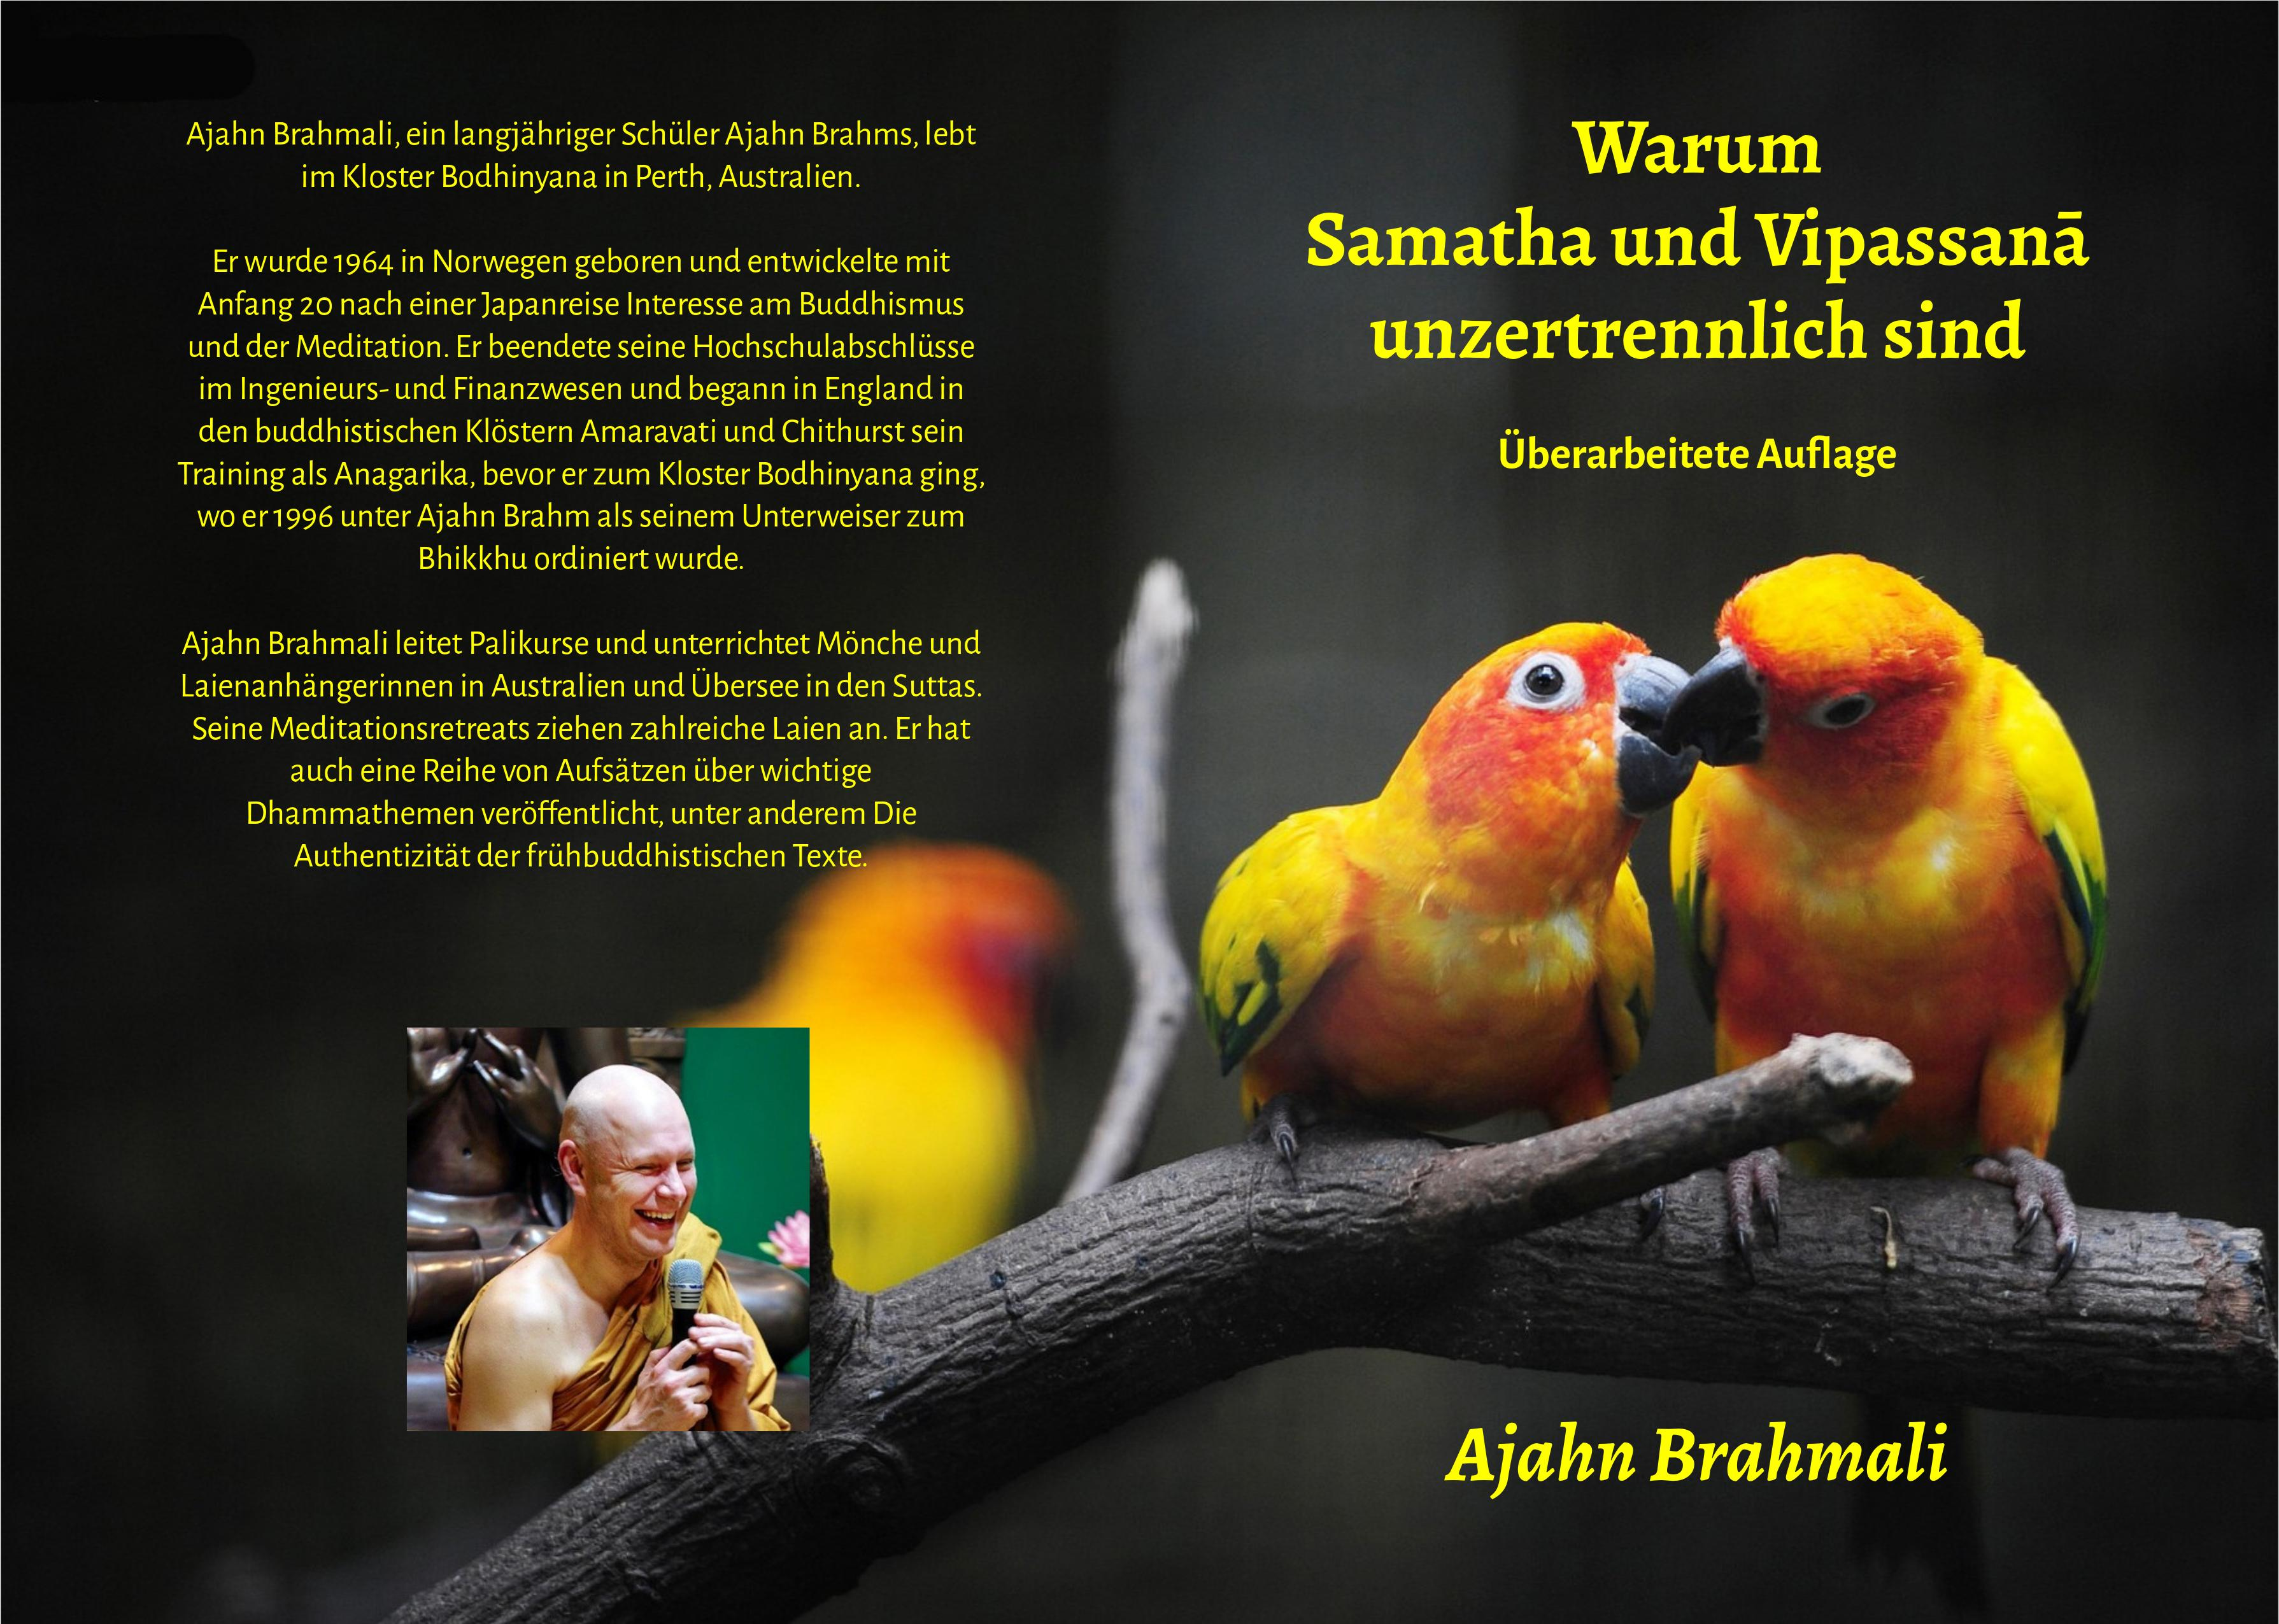
\includegraphics{sv-2_a5_cover_de-new}

\end{document}